\chapter{Vivado results}
After completing the verification phase, the circuit design was synthesized and implemented using the Vivado Tool, specifically targeting the Zybo Zynq-7010 development board.

\section{Vivado Design flow}
For the implementation of the CORDIC algorithm in vectoring mode for Cartesian-to-Polar conversion, the Vivado design flow was employed using Xilinx/AMD Vivado software. This process involved RTL Elaboration, Synthesis, and Implementation on the target FPGA, along with the application of design constraints and the extraction of power and timing reports. To ensure accurate and reliable timing analysis, all combinational logic paths were structured to follow a Register-Logic-Register configuration.

\section{RTL}
Vivado produced a logic network made of:

% todo cambiare numeri
\begin{enumerate}
    \item 144 cells (e.g. multiplexers, DFFs, adders)
    \item 68 I/O ports ($16_{x} + 16_{y} + 16_{\rho} + 16_{\theta} + 1_{clk} + 1_{rst} + 1_{start} + 1_{valid}$)
    \item 802 nets (for connecting all the components)
\end{enumerate}

The RTL Analysis generated the Elaborated Design shown in Figure \ref{fig:schematic}, consistent with the expected structure of the system.

\begin{figure}[H]
    \centering
    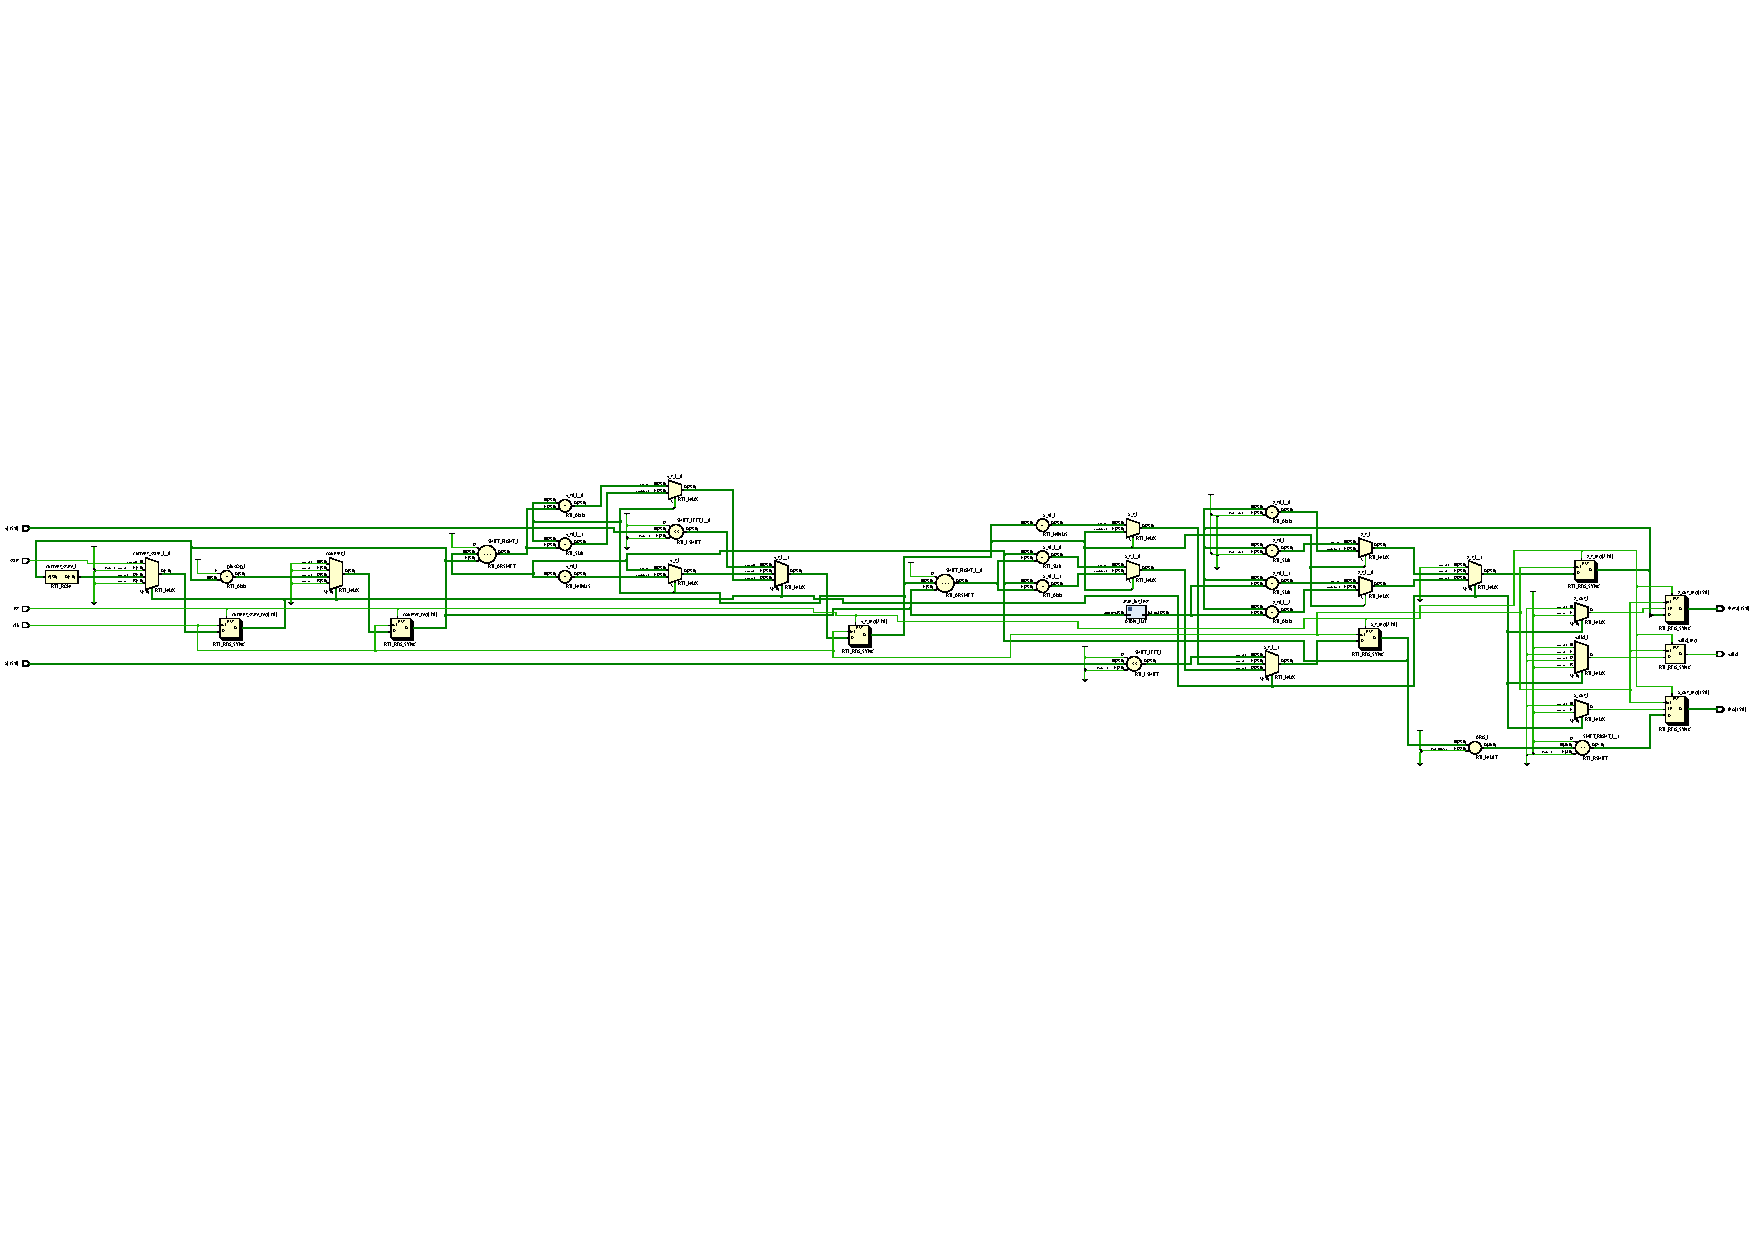
\includegraphics[width=\textwidth, trim=0 200 0 200, clip]{./images/Vivado/rtl.pdf}
    \caption{Elaborated RTL design.}
    \label{fig:schematic}
\end{figure}

\section{Synthesis timing report}
\begin{figure}[H]
    \centering
    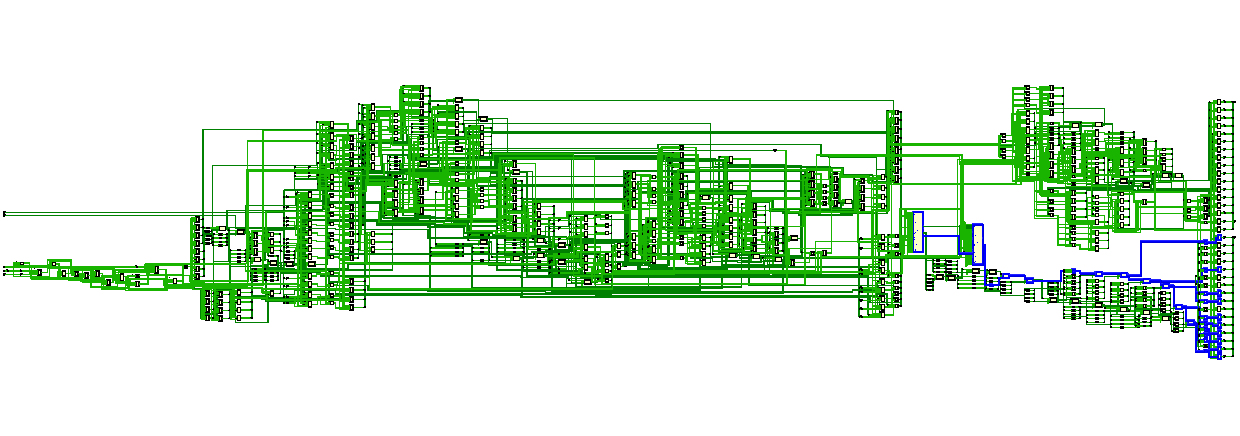
\includegraphics[width=\textwidth, trim=0 160 0 160, clip]{./images/Vivado/setup_synthesis.pdf}
    \caption{Figure showing the elaborated RTL design with the main critical paths for set-up-time-violation found in synthesis step highlighted in blue.}
    \label{fig:setup_synthesis}
\end{figure}

\begin{table}[H]
    \centering
    \small
    \captionsetup{skip=10pt} 
    \begin{tabular}{lrrrrrrr}
        \hline
        Name &  Slack &  Levels &  Routes & From      & To                 & Total Delay    \\
        \hline
        Path 1 &  12.78 &      10 &       6 & y\_t\_reg[14]/C  & ARG/A[23]       &         6.77   \\
        Path 2 &  12.78 &      10 &       6 & y\_t\_reg[14]/C  & ARG\_\_0/A[23]  &         6.77   \\
        Path 3 &  12.90 &       9 &       6 & y\_t\_reg[14]/C  & ARG/A[19]       &         6.66   \\
        Path 4 &  12.90 &       9 &       6 & y\_t\_reg[14]/C  & ARG\_\_0/A[19]  &         6.66   \\
        Path 5 &  13.02 &       8 &       6 & y\_t\_reg[14]/C  & ARG/A[15]       &         6.54   \\
        Path 6 &  13.02 &       8 &       6 & y\_t\_reg[14]/C  & ARG\_\_0/A[15]  &         6.54   \\
        Path 7 &  13.03 &      10 &       6 & y\_t\_reg[14]/C  & ARG/A[22]       &         6.53   \\
        Path 8 &  13.03 &      10 &       6 & y\_t\_reg[14]/C  & ARG\_\_0/A[22]  &         6.53   \\
        Path 9 &  13.08 &      10 &       6 & y\_t\_reg[14]/C  & ARG/A[21]       &         6.47   \\
        Path 10 &  13.08 &      10 &       6 & y\_t\_reg[14]/C  & ARG\_\_0/A[21]  &         6.47   \\
        \hline
    \end{tabular}
    \caption{Table showing data of the main critical paths found in synthesis step}
    \label{tab:setup_synthesis}
\end{table}
    
\begin{figure}[H]
    \centering
    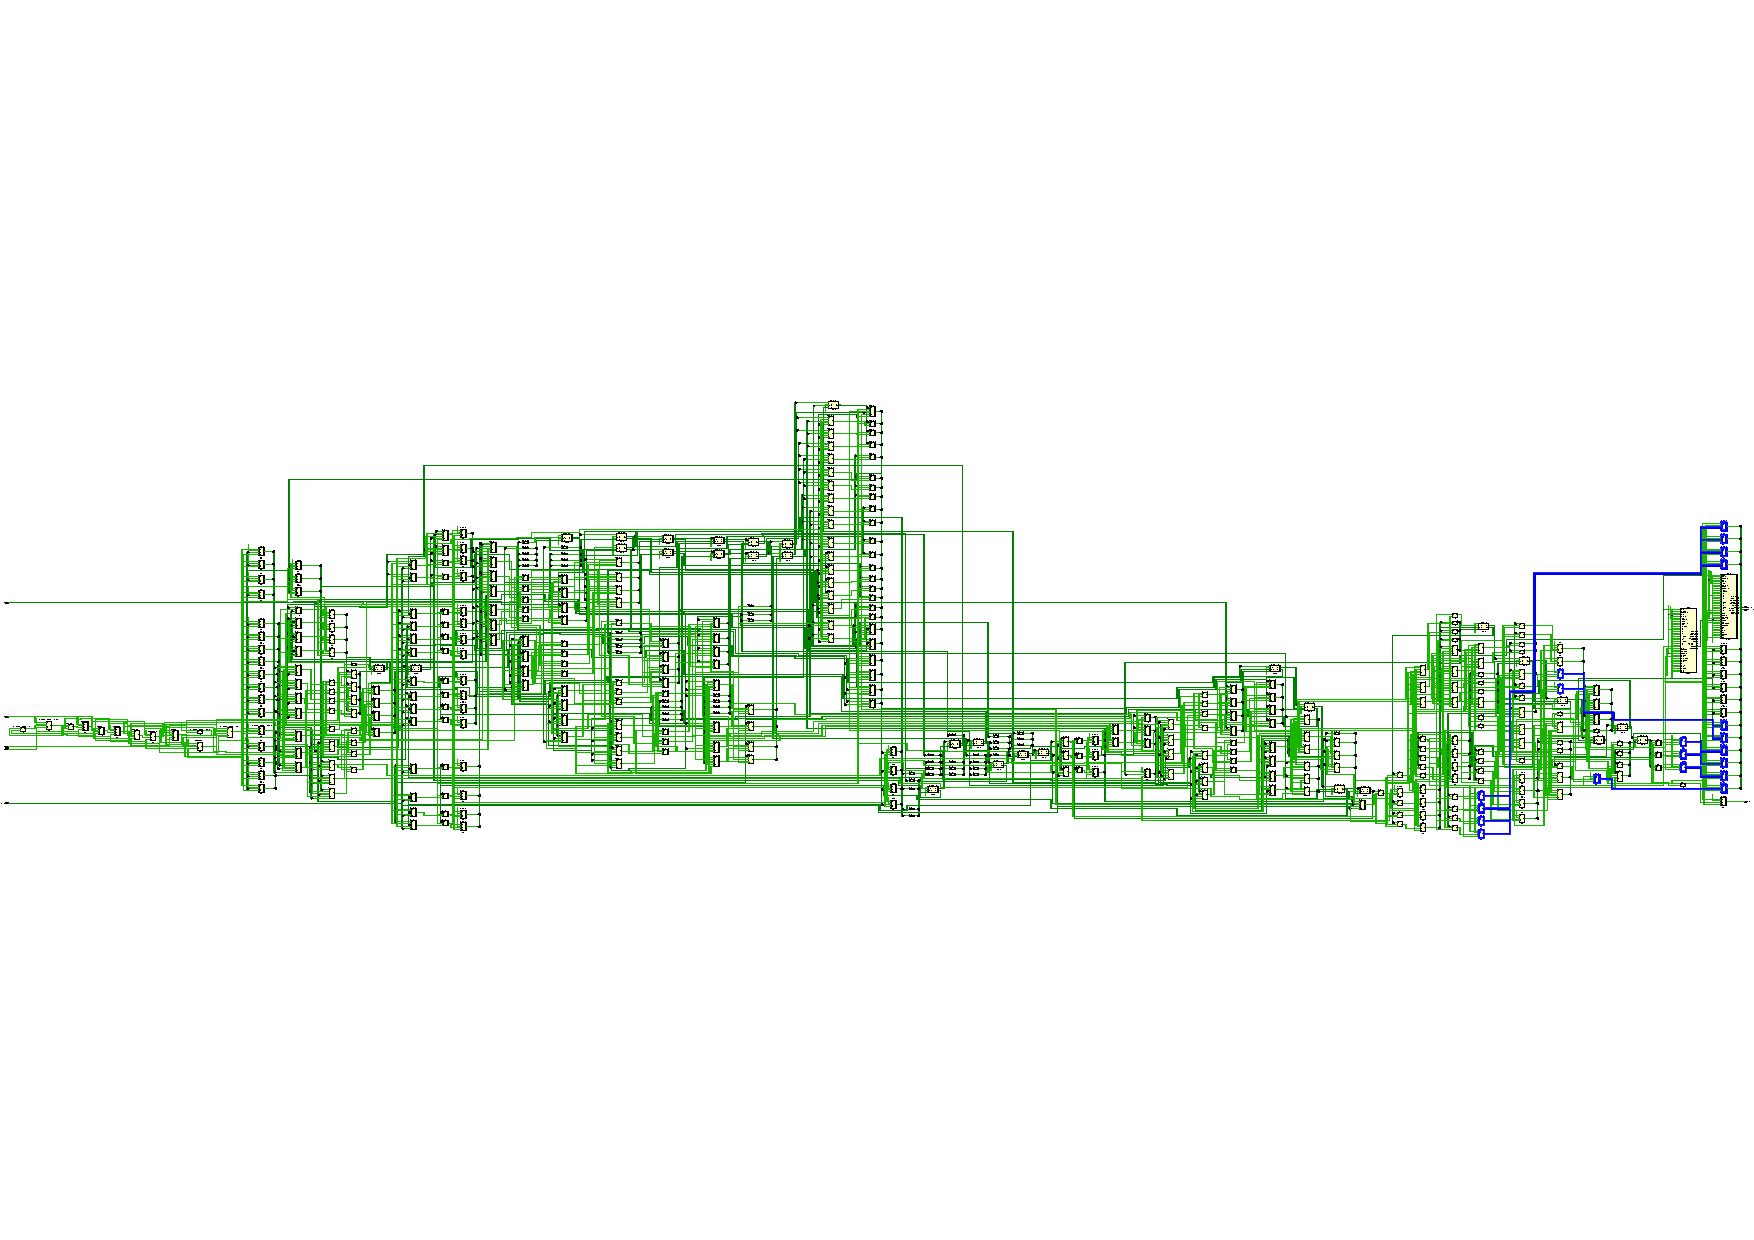
\includegraphics[width=\textwidth, trim=0 160 0 160, clip]{./images/Vivado/hold_synthesis.pdf}
    \caption{Figure showing the elaborated RTL design with the main critical paths for hold-time-violation found in synthesis step highlighted in blue.}
    \label{fig:hold_synthesis}
\end{figure}  

\begin{table}[H]
    \centering
    \small
    \captionsetup{skip=10pt} 
    \begin{tabular}{lrrrrrr}
        \hline
        Name    & Slack & Levels & Routes  & From           & To               & Total Delay \\
        \hline
        Path 11 &  0.28 &      0 &       1 & z\_t\_reg[23]/C & z\_out\_reg[15]/D & 0.30       \\
        Path 12 &  0.28 &      0 &       1 & z\_t\_reg[8]/C  & z\_out\_reg[0]/D  & 0.31       \\
        Path 13 &  0.28 &      0 &       1 & z\_t\_reg[18]/C & z\_out\_reg[10]/D & 0.31       \\
        Path 14 &  0.28 &      0 &       1 & z\_t\_reg[19]/C & z\_out\_reg[11]/D & 0.31       \\
        Path 15 &  0.28 &      0 &       1 & z\_t\_reg[20]/C & z\_out\_reg[12]/D & 0.31       \\
        Path 16 &  0.28 &      0 &       1 & z\_t\_reg[21]/C & z\_out\_reg[13]/D & 0.31       \\
        Path 17 &  0.28 &      0 &       1 & z\_t\_reg[22]/C & z\_out\_reg[14]/D & 0.31       \\
        Path 18 &  0.28 &      0 &       1 & z\_t\_reg[9]/C  & z\_out\_reg[1]/D  & 0.31       \\
        Path 19 &  0.28 &      0 &       1 & z\_t\_reg[10]/C & z\_out\_reg[2]/D  & 0.31       \\
        Path 20 &  0.28 &      0 &       1 & z\_t\_reg[11]/C & z\_out\_reg[3]/D  & 0.31       \\
        \hline
    \end{tabular}
    \caption{Table showing the characteristics regarding critical paths for hold-time-violation found in synthesis step.}
    \label{tab:hold_synthesis}
\end{table}



\section{Implementation timing report}

\begin{figure}[H]
    \centering
    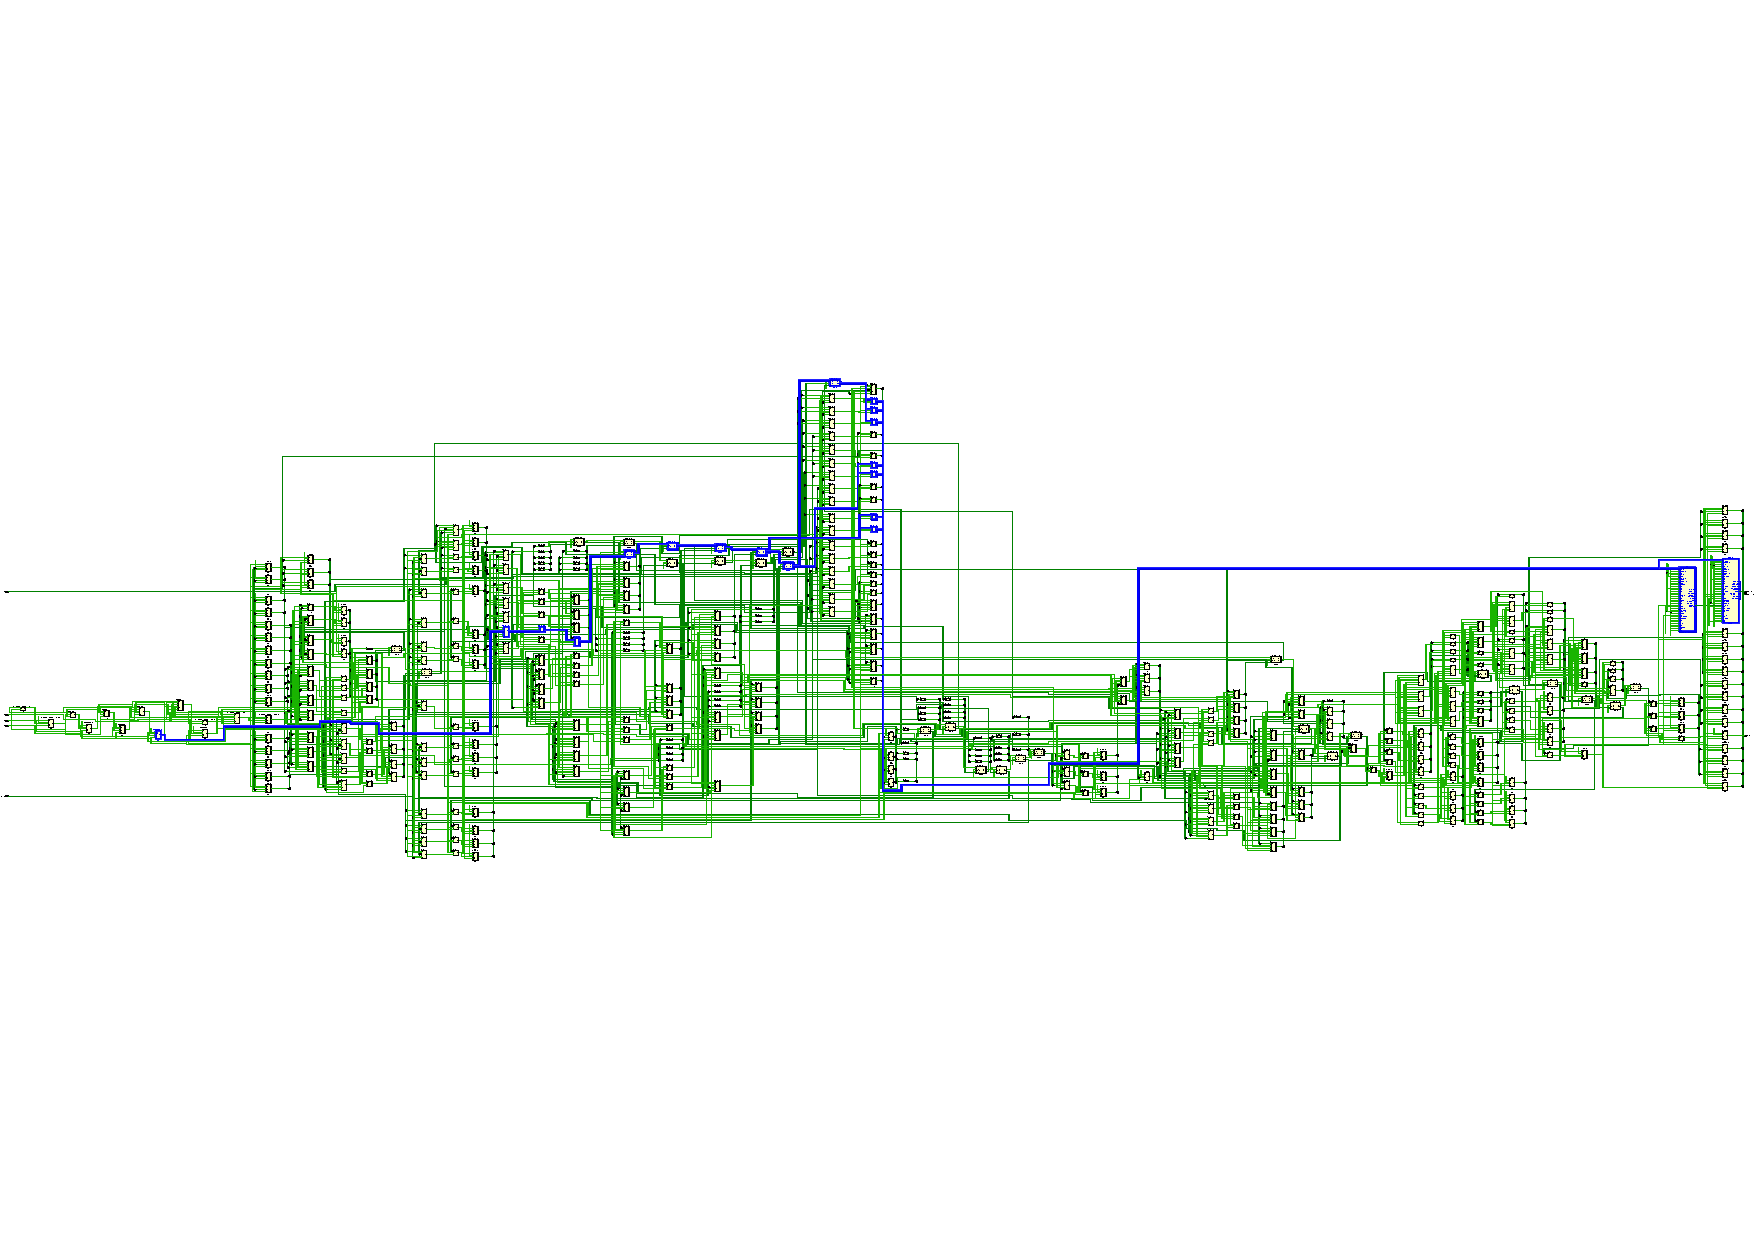
\includegraphics[width=\textwidth, trim=0 160 0 160, clip]{./images/Vivado/setup_implementation.pdf}
    \caption{Figure showing the elaborated RTL design with the main critical paths for set-up-time-violation found during implementation step highlighted in blue.}
    \label{fig:setup_implementation}
\end{figure}

\begin{table}[H]
    \centering
    \small
    \captionsetup{skip=10pt} 
    \begin{tabular}{lrrrrrr}
        \hline
        Name    & Slack & Levels & Routes  & From           & To               & Total Delay \\
        \hline
        Path 1  & 10.19 &      10 &       6 & counter\_reg[2]/C & ARG/A[20]        & 9.16       \\
        Path 2  & 10.38 &      10 &       6 & counter\_reg[2]/C & ARG\_\_0/A[20]   & 8.97       \\
        Path 3  & 10.43 &      10 &       6 & counter\_reg[2]/C & ARG\_\_0/A[21]   & 9.13       \\
        Path 4  & 10.43 &      10 &       6 & counter\_reg[2]/C & ARG/A[22]        & 8.92       \\
        Path 5  & 10.57 &       8 &       6 & counter\_reg[2]/C & ARG\_\_0/A[12]   & 8.78       \\
        Path 6  & 10.59 &       9 &       6 & counter\_reg[2]/C & ARG\_\_0/A[17]   & 8.97       \\
        Path 7  & 10.60 &       9 &       6 & counter\_reg[2]/C & ARG/A[16]        & 8.75       \\
        Path 8  & 10.61 &       8 &       6 & counter\_reg[2]/C & ARG\_\_0/A[13]   & 8.94       \\
        Path 9  & 10.61 &      10 &       6 & counter\_reg[2]/C & ARG/A[21]        & 8.94       \\
        Path 10 & 10.62 &      10 &       6 & counter\_reg[2]/C & ARG\_\_0/A[22]   & 8.73       \\
        \hline
    \end{tabular}
    \caption{Table showing the main critical paths for the setup-time-violation during the implementation step.}
    \label{tab:setup_implementation}
\end{table}

From the Table \ref{tab:setup_implementation} and the Figure \ref{fig:setup_implementation} we can notice that the main Critical Paths are due to the counter register that controls the logic of the iterative steps of the calculations. The worst negative slack (WNS) is 10.194ns indicating that the design can successfully operates at the 50MHz clock frequency with a large margin for an even faster clock.

\begin{figure}[H]
    \centering
    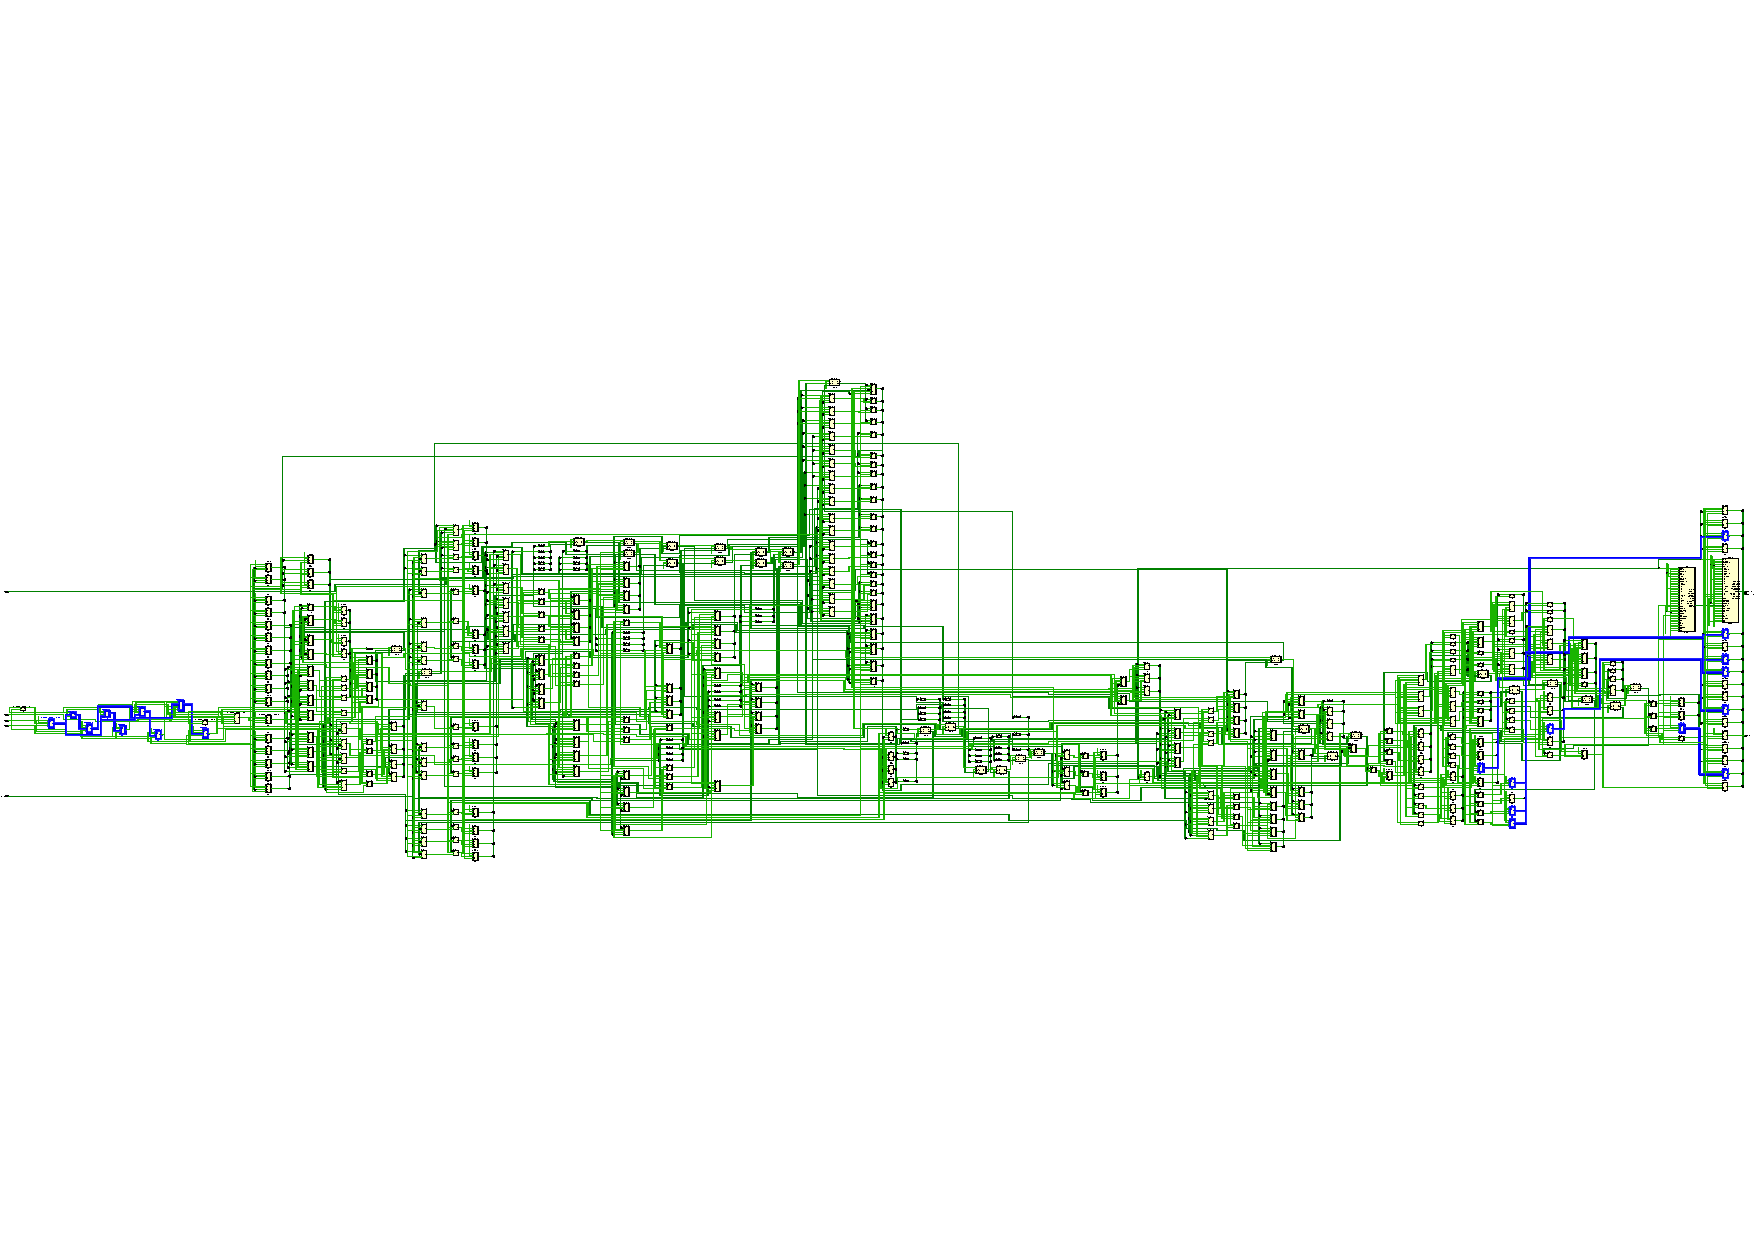
\includegraphics[width=\textwidth, trim=0 160 0 160, clip]{./images/Vivado/hold_implementation.pdf}
    \caption{Figure showing the elaborated RTL design with the main critical paths for hold-time-violation found during implementation step highlighted in blue.}
    \label{fig:hold_implementation}
\end{figure}

\begin{table}[H]
    \centering
    \small
    \captionsetup{skip=10pt} 
    \begin{tabular}{lrrrrrr}
        \hline
        Name    & Slack & Levels   & From                              & To                    & Total Delay \\
        \hline
        Path 11 &  0.17 &       1 &  current\_state\_reg[1]/C & counter\_reg[2]/D     & 0.33       \\
        Path 12 &  0.18 &       1 &  current\_state\_reg[1]/C & counter\_reg[0]/D     & 0.32       \\
        Path 13 &  0.18 &       1 &  current\_state\_reg[1]/C & counter\_reg[1]/D     & 0.32       \\
        Path 14 &  0.19 &       0 &  z\_t\_reg[22]/C                  & z\_out\_reg[14]/D     & 0.29       \\
        Path 15 &  0.22 &       0 &  z\_t\_reg[12]/C                  & z\_out\_reg[4]/D      & 0.29       \\
        Path 16 &  0.22 &       0 &  z\_t\_reg[14]/C                  & z\_out\_reg[6]/D      & 0.30       \\
        Path 17 &  0.23 &       0 &  z\_t\_reg[15]/C                  & z\_out\_reg[7]/D      & 0.26       \\
        Path 18 &  0.23 &       0 &  z\_t\_reg[10]/C                  & z\_out\_reg[2]/D      & 0.33       \\
        Path 19 &  0.24 &       1 &  counter\_reg[0]/C                & counter\_reg[3]/D     & 0.38       \\
        Path 20 &  0.24 &       0 &  z\_t\_reg[18]/C                  & z\_out\_reg[10]/D     & 0.32       \\
        \hline
    \end{tabular}
    \caption{Table showing the main critical paths for hold-time-violation found in the implementation step.}
    \label{tab:hold_implementation}
\end{table}

\section{Utilization Report}
\begin{table}[H]
    \centering
    \small
    \captionsetup{skip=10pt} 
    \begin{tabular}{lrr}
        \hline
        Resource               & Utilization (\%) & Description \\
        \hline
        Slice LUTs             & 1.59\%           & Look-Up Tables used as logic \\
        Slice Registers        & 0.27\%           & Registers used in the design \\
        Slice                  & 1.93\%           & Total slices utilized \\
        LUT as Logic           & 1.59\%           & LUTs specifically used as logic \\
        DSPs                   & 2.50\%           & Digital Signal Processing blocks \\
        Bonded IOB             & 0.00\%           & Bonded Input/Output Blocks \\
        BUFGCTRL               & 0.00\%           & Global Clock Buffers \\
        \hline
    \end{tabular}
    \caption{Resource utilization for the CORDIC design (only non-zero values shown)}
    \label{tab:cordic_resource_utilization}
\end{table}

From the Table \ref{tab:cordic_resource_utilization} we can notice that the utilization among the different FPGA resources is at most 2.5\%. This is perfectly compliant with the design objectives proposed in \ref{sec:algorithm_implementation}, where the CORDIC serves as an onboard accelerator, with area occupation as one of the key metrics.
\section{Power Report}
\begin{figure}[H]
    \centering
    \captionsetup{skip=10pt} 
    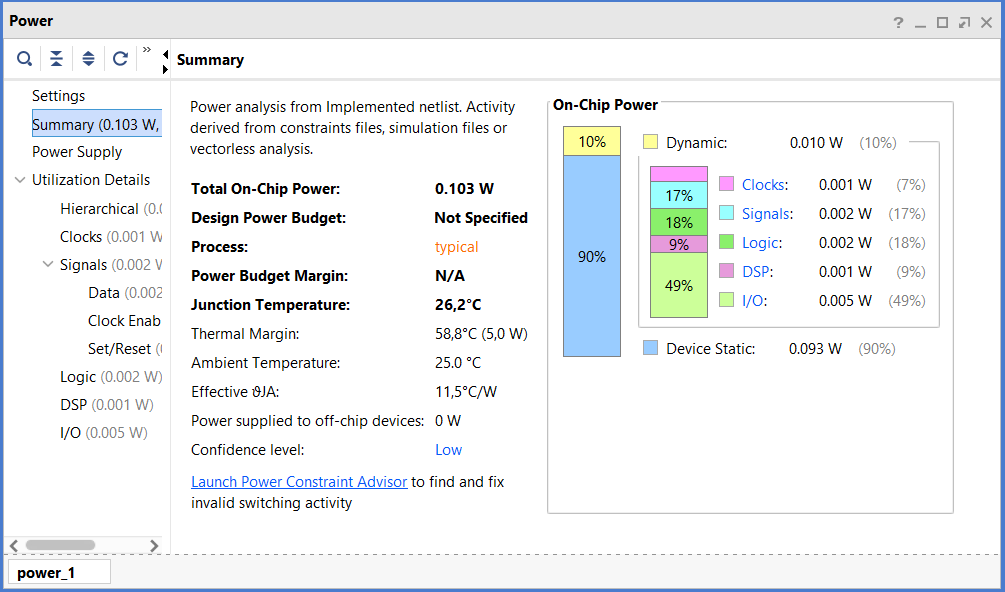
\includegraphics[width=\textwidth]{./images/Vivado/power_report.png}
    \caption{Vivado Power Report after implementation.}
    \label{fig:power_report}
\end{figure}
The power report highlights a total on-chip power consumption of 0.095 W, with 95\% attributed to static power (0.090 W) and 5\% to dynamic power (0.05 W). The dynamic power is distributed among different components: clocks (15\%), signals (31\%), logic (33\%), DSP (21\%), with signals and logic being the highest consumers of dynamic power.

The high value of static power over dynamic power is largely to be attributed to the fact that the design is using very little of the available hardware. With reference to the Utilization Report in Chapter \ref{chap:utlization_report}, resources like Slice LUTs and Registers are used only for 1.59\% and 0.27\%, this makes the overall switching activity of the chip very small.

This demonstrates that the power profile of the circuit is fully compliant with the objective of minimizing resource utilization and power consumption in an onboard accelerator scenario.

\section{Warnings}
During the implementation phase, various warnings were observed. These warnings arise from the fact that the design was developed in an out-of-context mode, which is standard practice for proof-of-concept implementations.

\begin{tcolorbox}[colback=yellow!20, colframe=yellow!50!black, title=Warnings]
\begin{itemize}
    \item \textbf{DRC 23-814} Not all possible (connectivity-based) DRCs may have been run because this design is seen as Out of Context.
    \item \textbf{Route 35-197} Clock port \texttt{"clk"} does not have an associated \texttt{HD.CLK\_SRC}. Without this constraint, timing analysis may not be accurate, and upstream checks cannot be done to ensure correct clock placement.
    \item \textbf{Route 35-198} Port \texttt{"rst"} does not have an associated \texttt{HD.PARTPIN\_LOCS}, which will prevent the partial routing of the signal \texttt{"rst"}. Without this partial route, timing analysis to/from this port will not be accurate, and no routing information for this port can be exported.
    \item \textbf{Timing 38-242} The property \texttt{HD.CLK\_SRC} of clock port \texttt{"clk"} is not set. In out-of-context mode, this prevents timing estimation for clock delay/skew.
\end{itemize}
\end{tcolorbox}

In our particular study case presented in Section \ref{sec:algorithm_implementation}, these warnings are not a cause for any concern. They arise because the design was intentionally tested in isolation, by just applying a single clock constraint with a 50MHz frequency. As a result, issues like incomplete connectivity checks and timing inaccuracies are reported.

Moreover, applying I/O pin constraints would be meaningless in this context. As discussed in \ref{sec:algorithm_implementation}, this device is intended to be an onboard accelerator for other circuits. Its primary purpose is to function as part of a larger system, and its inputs and outputs will be internally routed. Therefore, testing with external I/O constraints would not provide any meaningful insights.
